% éèàùôê
\chapter{Ordonnancement de tâches sur deux machines}

%%%%%%%%%%%%%%%%%%%%%%%%%%%%%%%%%%%%%%%%%%%%%%%%%%%%%%%%%%%%%%%%%%%%%%%%%%%%%%%%
%                                    TP 2                                      %
%%%%%%%%%%%%%%%%%%%%%%%%%%%%%%%%%%%%%%%%%%%%%%%%%%%%%%%%%%%%%%%%%%%%%%%%%%%%%%%%

\section{Problem statement}
\label{sec:enonce-du-probleme}

Consider a plant with two machines and to produce
parts. Each piece is the result of a sequence of tasks
takes place on one of the two machines. NB: machines are
specialized and can not be used interchangeably.


Each is described by its duration, the machine on which it
must be running and the list of preliminary tasks to be
completed before it starts. A task can at most
run on the same machine at a given time.

The problem is presented in the Figure ~\ref{opti}. Each node
represents one task. The values linked with the nodes are the task id and its duration. The tasks executed by the 1st machine are represented by a double circle. The others represent the tasks executed by the 2nd machine. The links represent the dependencies in between different tasks. A tack can only starts if all its previous dependencies have finished. The job is done when all tasks are done.

\begin{figure}
\begin{center}
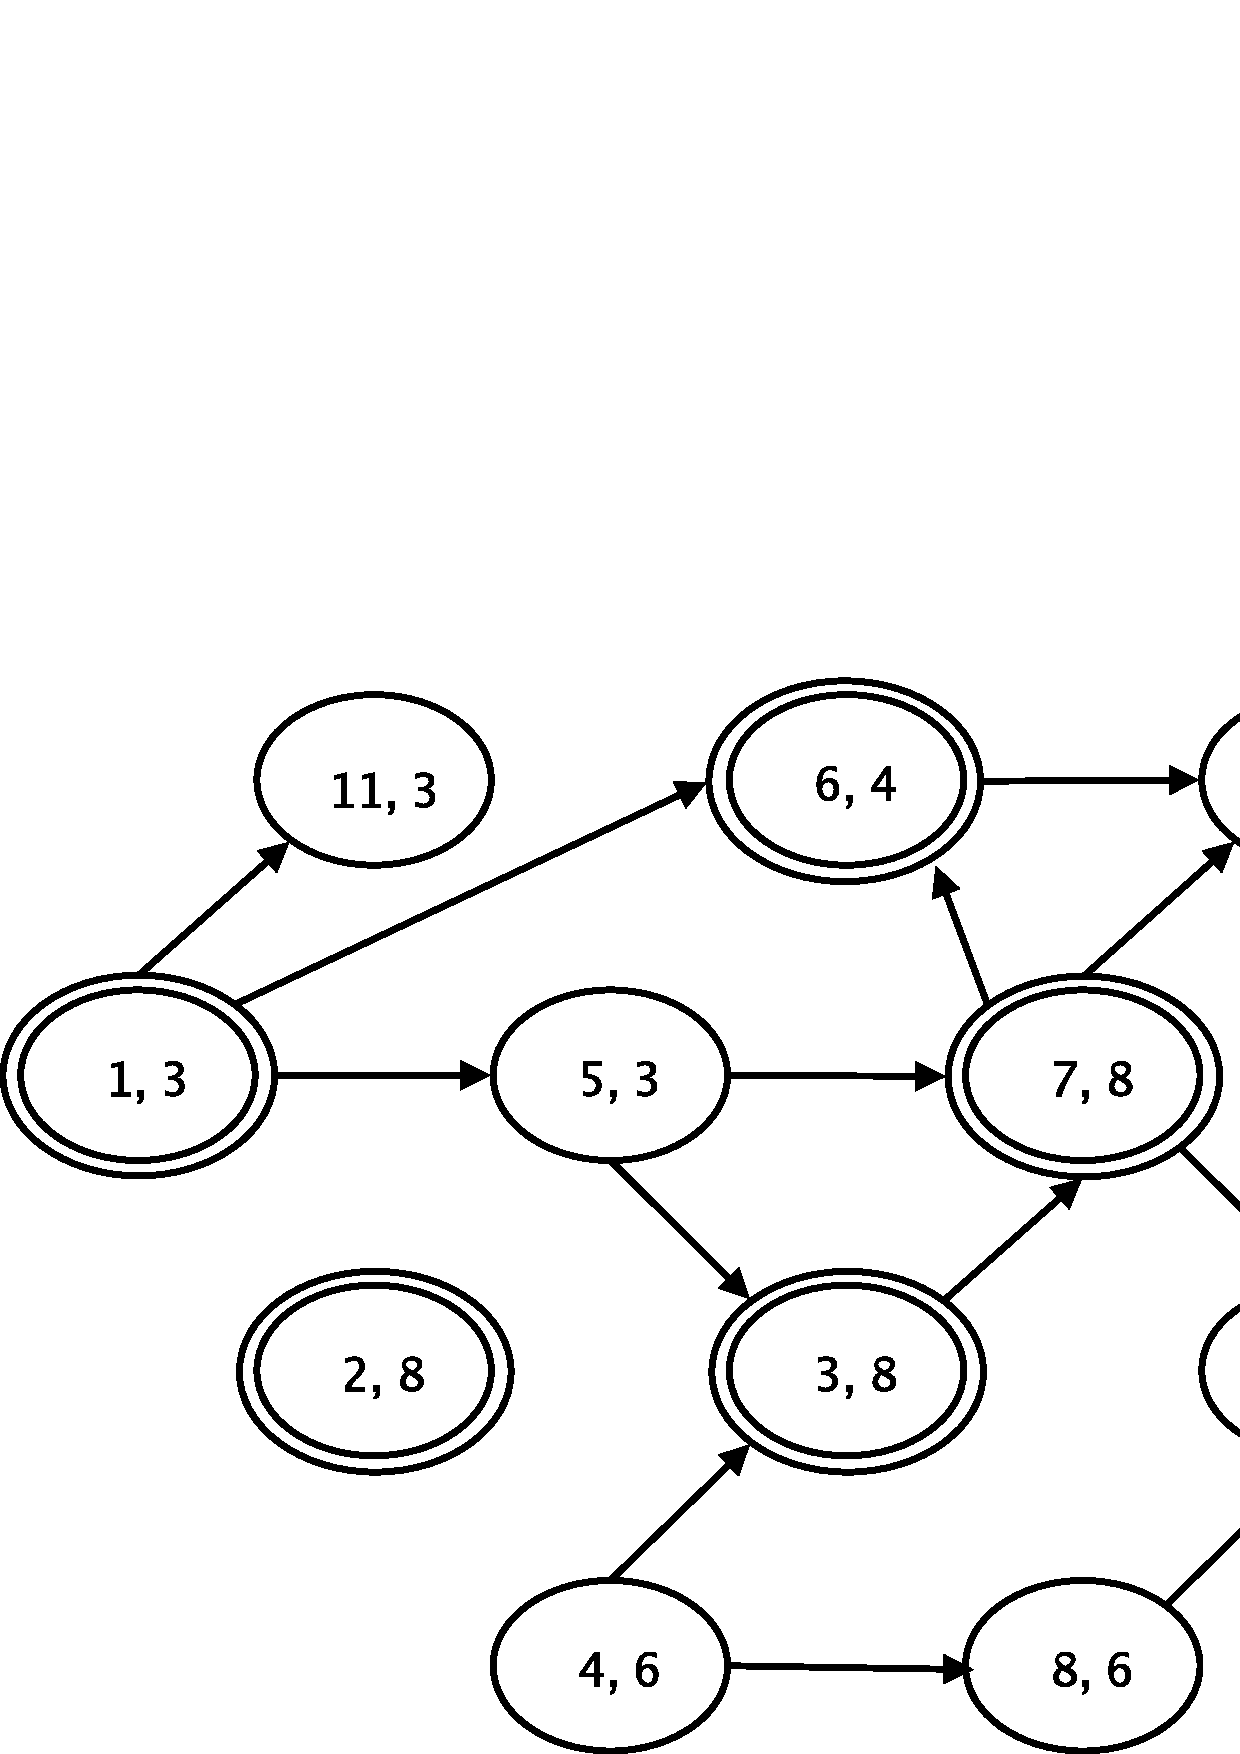
\includegraphics[width=7cm,height=5cm]{opti.pdf}
\caption{Dépendances entre les tâches}
\label{opti}
\end{center}
\end{figure}

This is to find start times for each task, in accordance with these constraints.
\section{Modélisation de la connaissance}
\label{sec:modelisation-connaissance}
We define a symbolic area for machine consists of two
values \verb|m1| and \verb|m2| (This allows the use of
symbolic constraints between variables representing
machines).
It represents a task by a term of the form:

\begin{center}
    \code{tache(Duree, Noms, Machine, Debut)},
\end{center}
where \code{Duree} is an integer giving the duration of the task in minutes
\code{Noms} is a list of clues preliminary tasks in the table
tasks,
 \code{Machine} is the name of the machine and \code{Debut} is a
variable representing the start date.
It represents the data and variables of the problem by an array of such

words:
\begin{center}
\begin{verbatim}
[](tache(3, [],     m1, _),
   tache(8, [],     m1, _),
   tache(8, [4,5],  m1, _),
   tache(6, [],     m2, _),
   tache(3, [1],    m2, _),
   tache(4, [1,7],  m1, _),
   tache(8, [3,5],  m1, _),
   tache(6, [4],    m2, _),
   tache(6, [6,7],  m2, _),
   tache(6, [9,12], m2, _),
   tache(3, [1],    m2, _),
   tache(6, [7,8],  m2, _))
\end{verbatim}
\end{center}

Note that in this problem, the machine that runs each task is known.

\section{Vers une solution en ECLiPSe}
\label{sec:vers-une-solutionOrdo}

\subsection{Une première solution partielle}
\begin{question} \label{TP2_Q1}
Define a predicate \code{taches(?Taches)} that unify \code{Taches} with a task table.
\end{question}

\begin{question}
  Set the iterator that retrieves each element and
   the poster. You will need this type of iterator for
   following questions.
\end{question}


\begin{question} \label{TP2_Q2}
Define a predicate \code{domaines(+Taches, ?Fin)} which requires that any task \code{Taches} starts after time 0 and
finish before the end of (additional variable corresponding to the moment when all tasks are completed).
\end{question}

\begin{question}
Define a predicate \code{getVarList(+Taches, ?Fin, ?List)} which allows to retrieve the list of variables from the problem.
\end{question}

\begin{question}
Define the predicate \code{solve(?Taches, ?Fin)} which uses the previous three predicates to find a schedule that respects the constraints of areas. Check that the solutions given by \eclipse{} are coherent.   
\end{question}

\subsection{Pose des contraintes d'ordonnancement}

NB: For the following two questions, test your
response using simple data.

\begin{question}
Define a predicate \code{precedences(+Taches)} qui contraint chaque tâche à démarrer après la fin de ses
tâches préliminaires. Modifiez \code{solve} pour prendre en compte ces contraintes et vérifiez que les nouvelles solutions proposées par \eclipse{} sont correctes.
\end{question}

\begin{question} \label{TP2_Q4}
Define a predicate\code{conflits(+Taches)} qui impose que, sur une machine, deux tâches ne se déroulent
pas en même temps. Modifiez \code{solve} pour obtenir une solution du problème prenant en compte cette dernière contrainte.
\end{question}

\subsection{La meilleure solution ?}

In this problem, there is a notion of relative quality of
solutions: if a solution $S_1$ is such that the value of
\code{Fin} is less than that of the solution $S_2$, then $S_1$
is better than $S_2$.  We can be interested in the research
the best solution of the problem or the best
solutions.
\begin{question} \label{TP2_last}
 Do you think the solution found by eclipse is the best solution? If so, explain why. Otherwise modify your code to find an optimal solution.
\end{question}


% \section{Optimisation}
% 
% \subsection{Branch and bound dans ic}
% Pour faire de l'optimisation dans le cadre des contraintes à domaine
% finis, le principe de \emph{branch and bound} est généralement
% utilisé. En ECLiPSe, le prédicat \verb|min_max/2| est une
% instanciation de ce principe basée sur la propagation de
% contraintes. Le premier paramètre est un but. Ce but génère un arbre
% de recherche. Le deuxième paramètre est une variable à
% minimiser. \verb|min_max/2| réalise un parcours « intelligent » de
% l'arbre de recherche pour trouver la feuille de l'arbre où la borne
% inférieure du domaine de la variable à minimiser est la plus petite et
% retourne cette borne inférieure. Par conséquent, il faut toujours
% faire un labeling dans le but passé en paramètre de min\_max, sinon la
% valeur rendue peut ne pas correspondre à une solution du problème à
% contraintes. L'exemple suivant
% illustre cette propriété : \verb|[X,Y,Z] :: 1..10, X #= Y+Z, X #= Y*Z|\\
% Utilisez \verb|min_max/2| pour trouver la plus petite valeur de $X$
% solution de ce problème (regardez le manuel d'ECLiPSe pour une
% présentation de min\_max plus approfondie). Essayez sans labeling puis
% avec.
% 
% \begin{question}
% Expliquez les deux valeurs différentes rendues par ECLiPSe.
% \end{question}
% 
% \subsection{Le meilleur ordonnancement}
% \begin{question} \label{TP2_Q6}
% Adresser les requêtes pour trouver un ordonnancement optimal (qui termine au
% plus tôt) et qui respecte les contraintes.
% \end{question}

\section{Compte-rendu}

\subsection{À rendre}

\begin{enumerate}
\item The code \eclipse{} \emph{commenté}. Give eclipse requests
   used to test each question and test data when the data are not the problem.
   For each request, also give the system responses.
\item The detailed answer to the question~\ref{TP2_last} 
\end{enumerate}


